%%%%%%%%%%%%%%%%%%%%%%%%%%%%%%%%%%%%%%%%%
% Beamer Presentation
% LaTeX Template
% Version 1.0 (10/11/12)
%
% This template has been downloaded from:
% http://www.LaTeXTemplates.com
%
% License:
% CC BY-NC-SA 3.0 (http://creativecommons.org/licenses/by-nc-sa/3.0/)
%
%%%%%%%%%%%%%%%%%%%%%%%%%%%%%%%%%%%%%%%%%

%----------------------------------------------------------------------------------------
%	PACKAGES AND THEMES
%----------------------------------------------------------------------------------------

\documentclass{beamer}

\mode<presentation> {

% The Beamer class comes with a number of default slide themes
% which change the colors and layouts of slides. Below this is a list
% of all the themes, uncomment each in turn to see what they look like.

%\usetheme{default}
%\usetheme{AnnArbor}
%\usetheme{Antibes}
%\usetheme{Bergen}
%\usetheme{Berkeley}
%\usetheme{Berlin}
%\usetheme{Boadilla}
%\usetheme{CambridgeUS}
%\usetheme{Copenhagen}
%\usetheme{Darmstadt}
%\usetheme{Dresden}
%\usetheme{Frankfurt}
%\usetheme{Goettingen}
%\usetheme{Hannover}
%\usetheme{Ilmenau}
%\usetheme{JuanLesPins}
%\usetheme{Luebeck}
\usetheme{Madrid}
%\usetheme{Malmoe}
%\usetheme{Marburg}
%\usetheme{Montpellier}
%\usetheme{PaloAlto}
%\usetheme{Pittsburgh}
%\usetheme{Rochester}
%\usetheme{Singapore}
%\usetheme{Szeged}
%\usetheme{Warsaw}

% As well as themes, the Beamer class has a number of color themes
% for any slide theme. Uncomment each of these in turn to see how it
% changes the colors of your current slide theme.

%\usecolortheme{albatross}
%\usecolortheme{beaver}
%\usecolortheme{beetle}
%\usecolortheme{crane}
%\usecolortheme{dolphin}
%\usecolortheme{dove}
%\usecolortheme{fly}
%\usecolortheme{lily}
%\usecolortheme{orchid}
%\usecolortheme{rose}
%\usecolortheme{seagull}
%\usecolortheme{seahorse}
%\usecolortheme{whale}
%\usecolortheme{wolverine}

%\setbeamertemplate{footline} % To remove the footer line in all slides uncomment this line
%\setbeamertemplate{footline}[page number] % To replace the footer line in all slides with a simple slide count uncomment this line

%\setbeamertemplate{navigation symbols}{} % To remove the navigation symbols from the bottom of all slides uncomment this line
}

\usepackage{graphicx} % Allows including images
\usepackage{booktabs} % Allows the use of \toprule, \midrule and \bottomrule in tables
\usepackage{listings}
\usepackage{amsmath}
\usepackage{algpseudocode,algorithm,algorithmicx}

\lstdefinestyle{customjava}{
  breaklines=true,
  frame=L,
  xleftmargin=\parindent,
  language=Java,
  showstringspaces=false,
  basicstyle=\footnotesize\ttfamily,
  keywordstyle=\bfseries\color{green!40!black},
  commentstyle=\itshape\color{gray!40!black},
  identifierstyle=\color{blue},
  stringstyle=\color{orange},
}

%----------------------------------------------------------------------------------------
%	TITLE PAGE
%----------------------------------------------------------------------------------------

\title[Multimedia Data]{Multimedia Data} % The short title appears at the bottom of every slide, the full title is only on the title page

\author{Jonathan Windle} % Your name
\institute[UEA] % Your institution as it will appear on the bottom of every slide, may be shorthand to save space
{
University of East Anglia \\ % Your institution for the title page
\medskip
\textit{J.Windle@uea.ac.uk} % Your email address
}
\date{\today} % Date, can be changed to a custom date

\begin{document}

\begin{frame}
\titlepage % Print the title page as the first slide
\end{frame}

\begin{frame}[allowframebreaks]
\frametitle{Overview} % Table of contents slide, comment this block out to remove it
\tableofcontents % Throughout your presentation, if you choose to use \section{} and \subsection{} commands, these will automatically be printed on this slide as an overview of your presentation
\end{frame}

%------------------------------------------------------------------
\section{Requirements of Applications}
\begin{frame}
\frametitle{Requirements of Applications}
\begin{itemize}
\item \textbf{Speech:} Needs to be sent in real-time for conversations but relatively low in terms of bit rate. Speech can also tolerate errors and to some extent the speech coding algorithm can hide them.
\item \textbf{Audio streaming:} Needs to be fast, but not necessarily real-time - can employ buffering on the termincal to allow for variability in transmission times.. Can also tolerate errors and to some extend can hide them.
\item \textbf{images:} Have no real-time requirement but can often be quite large in size. Can tolerate a small number of errors in transmission.
\item \textbf{Video phone:} Needs to be real-time while video streaming does not. High bit rate requirements and error tolerant.
\item \textbf{SMS:} Does not need to be real time or require large bit rates, however the messages are not error tolerant.
\end{itemize}
\end{frame}
%----------------------------------------------------------------
\section{Application Service Requirements - Transport Layer}
\begin{frame}
\frametitle{Application Service Requirements - Transport Layer}
\begin{itemize}
\item \textbf{Throughput:} Required data transfer rate - bits per second - to support the application.
\item \textbf{Latency:} Maximum propogation delay/maximum variation to make application usable. 
\item \textbf{Error Sensitivity:} How sensitive the application is to errors in the data.
\end{itemize}
\end{frame}
%----------------------------------------------------------------
\section{Circuit switched vs Packet switched}
\begin{frame}[allowframebreaks]
\frametitle{Circuit switched vs Packet switched}
\begin{itemize}
\item {\color{red}Circuit Switched:}
\begin{itemize}
\item Require dedicated point-to-point connections during call.
\item Continuous stream of data
\item E.G. Phone network.
\item Physical circuit allocated for each connection.
\item If insufficient resources are available then the connection is refused (e.g. engaged signal)
\item If an invalid number is called then you hear the unobtainable tone
\end{itemize}
\item {\color{green}Packet Switched:}
\begin{itemize}
\item Move data in seperate, small blocks.
\item Each packet contains destination address.
\item Packets reassembled in sequence make up the message.
\item Example is IP network.
\item Address field of header is used to decide path through the network.
\item Packets may take different routes though
\item Network will always attempt to deliver the packets even in times of congestion.
\end{itemize}
\end{itemize}
Circuit
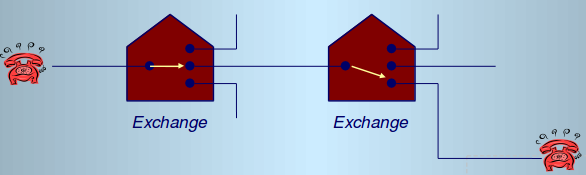
\includegraphics[scale=0.4]{circuit.png}\\
Switched
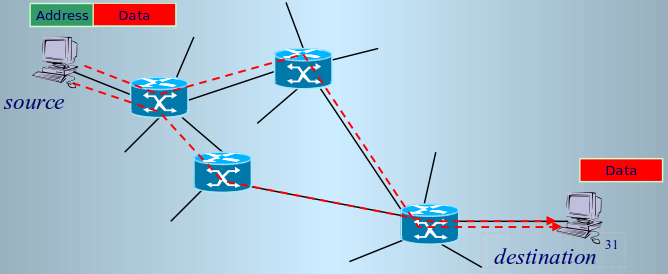
\includegraphics[scale=0.4]{switched.png}
\end{frame}
%------------------------------------------------------------------
\section{Connection-oriented and connectionless}
\begin{frame}
\frametitle{Connection-oriented and connectionless}
\begin{itemize}
\item {\color{red}Connection-oriented:}
\begin{itemize}
\item Requires connection set-up and close-down.
\item Packets are acknowledged by the receiver.
\item If no acknowledgement by the receiver then the packet is re-sent.
\item Guaranteed in-order delivery of packets.
\item In the IP suite this service is provided by the {\color{purple} Transmission Control Protocol} (TCP).
\end{itemize}
\item {\color{green}Connectionless:}
\begin{itemize}
\item No connection set-up or close-down.
\item No guarantee of delivery.
\item No acknowledgement of receipt.
\item No in-order delivery
\item Packets transmitted in isolation, delivered on a best effort basis.
\item In the IP suite this service is provided by the {\color{orange} User Datagram Protocol} (UDP).
\end{itemize}
\end{itemize}
\end{frame}
%-----------------------------------------------------------------
\begin{frame} 
\Huge{\centerline{The End}}
\end{frame}
\end{document}